% ============================================================
% v1.0.14 P5.1 Step 33 편입 — 원본(치환 전) figure 블록 보존
% graphite_ica_ch1_v1.0.14.tex 에서 T1..T8 승자 편입 시 삭제된 원본
% 대상 순서(T1..T8)대로 append. 각 블록 앞에 라벨 주석.
% ============================================================

% ---- T1 (fig:spine) 원본 — 원 위치: ch1.tex L158-191 ----
\begin{figure}[t]
\centering
\begin{tikzpicture}[
  node distance=4.3mm and 5.5mm,
  stage/.style={draw,rounded corners=2pt,minimum height=7.4mm,inner xsep=4pt,inner ysep=2.5pt,font=\scriptsize,align=center,fill=black!4},
  core/.style={stage,fill=black!10},
  io/.style={font=\scriptsize\itshape,align=center},
  ar/.style={-{Latex[length=1.6mm]},thick}]
% input row
\node[io] (in) {input: $V_\app$, direction $\to\sigma_d$, c-rate $\to|I|$, $T$, $Q_\cell$};
% spine
\node[stage,below=5mm of in] (n0) {N0\\map inputs};
\node[stage,below=of n0] (n1) {N1: polarization\\$V_n=V_\app-\sigma_d|I|R_n$};
\node[stage,below=of n1] (n2) {N2: center\\$U_j(T)=(-\Delta H+T\Delta S)/F$};
\node[stage,below=of n2] (n3) {N3: hysteresis branch\\center $\to U_j+\tfrac12\sigma_d h_\eta\gamma\,\Delta U_\hys$};
\node[stage,below=of n3] (n4) {N4/N5: width $w$, $\xi_\eq$\\$\xi_\eq=\mathrm{logistic}[\sigma_d(V-U)/w]$};
\node[stage,below=of n4] (n6) {N6: equilibrium peak\\$Q_j\,\xi_\eq(1-\xi_\eq)/w$};
\node[stage,below=of n6] (n7) {N7: lag length $L_V$\\$A,\chi_d,\Delta H_a^\eff,L_q,L_V$};
\node[stage,below=of n7] (n8) {N8: causal memory tail\\$(\xi_\eq-\xi_\mathrm{lag})/L_V$, charge reversal};
\node[core,below=of n8] (n9) {N9: sum + interp\\$C_\bg+\sum_j Q_j[\cdot]$};
\node[io,below=4.5mm of n9] (out) {output: $\dd Q/\dd V$ at $V_n$};
\foreach \a/\b in {in/n0,n0/n1,n1/n2,n2/n3,n3/n4,n4/n6,n6/n7,n7/n8,n8/n9,n9/out}
  \draw[ar] (\a) -- (\b);
% per-transition loop bracket
\begin{scope}[on background layer]
\node[draw,dashed,rounded corners,fit=(n2)(n3)(n4)(n6)(n7)(n8),inner sep=3.4mm,label={[font=\scriptsize\itshape,anchor=north west]north west:per-transition loop $j=1..N_p$}] (loop) {};
\end{scope}
\end{tikzpicture}
\caption{한 곡선을 그리는 계산 진행(spine). 외부 실험조건 $(\sigma_d,|I|,T,Q_\cell)$
이 N0 에서 모델 입력으로 환산되고, 분극으로 내부 전위 $V_n$ 을 얻은 뒤(N1), 전이 $j$ 마다 평형 중심$\cdot$히스
분기$\cdot$폭$\cdot$평형 진행률$\cdot$평형 peak$\cdot$지연 길이$\cdot$인과 꼬리를 계산해(N2--N8) 합산$\cdot$역보간한다(N9).
파선 상자는 전이별 반복 계산 단위다.}
\label{fig:spine}
\end{figure}

% ---- T2 (fig:staging) 원본 — 원 위치: ch1.tex L272-305 ----
\begin{figure}[t]
\centering
\begin{tikzpicture}[x=1.05cm,y=0.5cm,
  lab/.style={font=\scriptsize,align=center},
  fill4/.style={fill=black!72},fillL/.style={fill=black!24}]
% five stage columns, each shows graphene layers (lines) and Li-filled galleries (bands)
% column x-centers
\def\colw{0.85}
% stage 4: 1 filled gallery of 4
\foreach \x/\name/\filled/\style in {0/{stage 4}/{1}/fill4, 1.4/{stage 3}/{1}/fill4, 2.8/{stage 2L}/{all}/fillL, 4.2/{stage 2}/{all}/fill4, 5.6/{stage 1}/{dense}/fill4}{
  \draw[semithick] (\x,0)--(\x+\colw,0);
  \foreach \k in {1,2,3,4,5,6}{\draw[semithick] (\x,0.6*\k)--(\x+\colw,0.6*\k);}
  \node[lab,below] at (\x+\colw/2,-0.25) {\name};
}
% galleries (bands between layers) — explicit per column for clarity
% stage 4: every 4th gallery filled
\foreach \k in {1,5}{\fill[black!72] (0,0.6*\k-0.42) rectangle (0+\colw,0.6*\k-0.18);}
% stage 3: every 3rd
\foreach \k in {1,4}{\fill[black!72] (1.4,0.6*\k-0.42) rectangle (1.4+\colw,0.6*\k-0.18);}
% stage 2L: every 2nd, light (liquid-like)
\foreach \k in {1,3,5}{\fill[black!24] (2.8,0.6*\k-0.42) rectangle (2.8+\colw,0.6*\k-0.18);}
% stage 2: every 2nd, dark
\foreach \k in {1,3,5}{\fill[black!72] (4.2,0.6*\k-0.42) rectangle (4.2+\colw,0.6*\k-0.18);}
% stage 1: all galleries
\foreach \k in {1,2,3,4,5,6}{\fill[black!72] (5.6,0.6*\k-0.42) rectangle (5.6+\colw,0.6*\k-0.18);}
\draw[-{Latex[length=1.8mm]},thick] (0,4.05)--(6.45,4.05) node[pos=0.5,above,font=\scriptsize] {lithiation (charge): $4\to3\to2\mathrm L\to2\to1$};
\draw[{Latex[length=1.8mm]}-,thick] (0,-1.05)--(6.45,-1.05) node[pos=0.5,below,font=\scriptsize] {delithiation (discharge): main direction, $\theta_j:1\to0$};
\end{tikzpicture}
\caption{흑연 staging 의 갤러리 채움 도식. 수평선이 그래핀 층, 음영 띠가 리튬이 든 층간 갤러리다.
채울수록 stage 번호가 줄어 stage 1($\mathrm{LiC_6}$, 완전 채움)에 닿고, 각 stage 전이가 $\dd Q/\dd V$ 에 peak
하나를 남긴다. stage $2\mathrm L$ 은 면내 질서가 풀린 단계라 옅게 표시했다. 코드의 전이 리스트 4건이 이 전이들의
초기값이며($U\approx0.21/0.14/0.12/0.085$ V), 본 문건 방향은 방전(탈리튬화)이다.}
\label{fig:staging}
\end{figure}

% ---- T3 (fig:hysloop) 원본 — 원 위치: ch1.tex L1147-1173 ----
\begin{figure}[t]
\centering
\begin{tikzpicture}[x=9.2cm,y=1.7cm]
\draw[-{Latex[length=1.6mm]}] (0,-1.45) -- (0,1.55) node[left,font=\scriptsize] {$(sF/RT)(V_\eq-U_j)$};
\draw[-{Latex[length=1.6mm]}] (-0.02,0) -- (1.06,0) node[below,font=\scriptsize] {$\xi$};
\foreach \xx in {0.25,0.5,0.75} {\draw (\xx,0.03) -- (\xx,-0.03) node[below,font=\scriptsize] {\xx};}
% non-monotone V_eq(xi) for Omega=4RT — exact 4dp: y = ln[xi/(1-xi)] + 4(1-2 xi)
\draw[thick] plot[smooth] coordinates {(0.02,-0.0518) (0.05,0.6556) (0.08,0.9177) (0.1,1.0028) (0.1464,1.0657) (0.2,1.0137) (0.3,0.7527) (0.4,0.3945) (0.5,0) (0.6,-0.3945) (0.7,-0.7527) (0.8,-1.0137) (0.8536,-1.0657) (0.9,-1.0028) (0.92,-0.9177) (0.95,-0.6556) (0.98,0.0518)};
\fill (0.1464,1.0657) circle (0.5pt) node[above,font=\scriptsize] {$\xi_s^-$};
\fill (0.8536,-1.0657) circle (0.5pt) node[below,font=\scriptsize] {$\xi_s^+$};
\draw[{Latex[length=1.4mm]}-{Latex[length=1.4mm]}] (1.0,-1.0657) -- (1.0,1.0657) node[pos=0.4,right,font=\scriptsize] {$\Delta U_j^\hys$};
% discharge overshoot path (rising branch up to xi_s^-)
\draw[-{Latex[length=1.6mm]},very thick] plot[smooth] coordinates {(0.02,-0.0518) (0.05,0.6556) (0.08,0.9177) (0.1,1.0028) (0.1464,1.0657)};
\draw[-{Latex[length=1.4mm]},densely dashed] (0.1464,1.0) -- (0.1464,0.08);
\node[font=\scriptsize] at (0.32,1.30) {discharge overshoot};
% charge overshoot path
\draw[-{Latex[length=1.6mm]},very thick] plot[smooth] coordinates {(0.98,0.0518) (0.95,-0.6556) (0.92,-0.9177) (0.9,-1.0028) (0.8536,-1.0657)};
\draw[-{Latex[length=1.4mm]},densely dashed] (0.8536,-1.0) -- (0.8536,-0.08);
\node[font=\scriptsize] at (0.68,-1.30) {charge overshoot};
\node[font=\scriptsize] at (0.24,-0.55) {$\gamma\!\to\!0$: plateau at $U_j$ ($y=0$)};
\end{tikzpicture}
\caption{비단조 평형 전위 $V_\eq(\xi)$(식~\eqref{eq:Veq}, $\Omega_j=4RT$ — 좌표는 식 그대로의 수치 평가)와 과주행. 방전(굵은 경로,
좌상)은 극대 $\xi_s^-$ 까지, 충전(우하)은 극소 $\xi_s^+$ 까지 과주행해 중심이 갈라진다. 두 극값 차가 spinodal 상한
gap $\Delta U_j^\hys$(식~\eqref{eq:dUhys}), 실측 분기는 $\gamma_j$ 만큼 안쪽(식~\eqref{eq:Ubranch}). $\gamma\to0$
가역 한계에서 두 경로가 $y=0$ plateau 로 합쳐진다.}
\label{fig:hysloop}
\end{figure}

% ---- T4 (fig:barrier) 원본 — 원 위치: ch1.tex L1255-1289 ----
\begin{figure}[t]
\centering
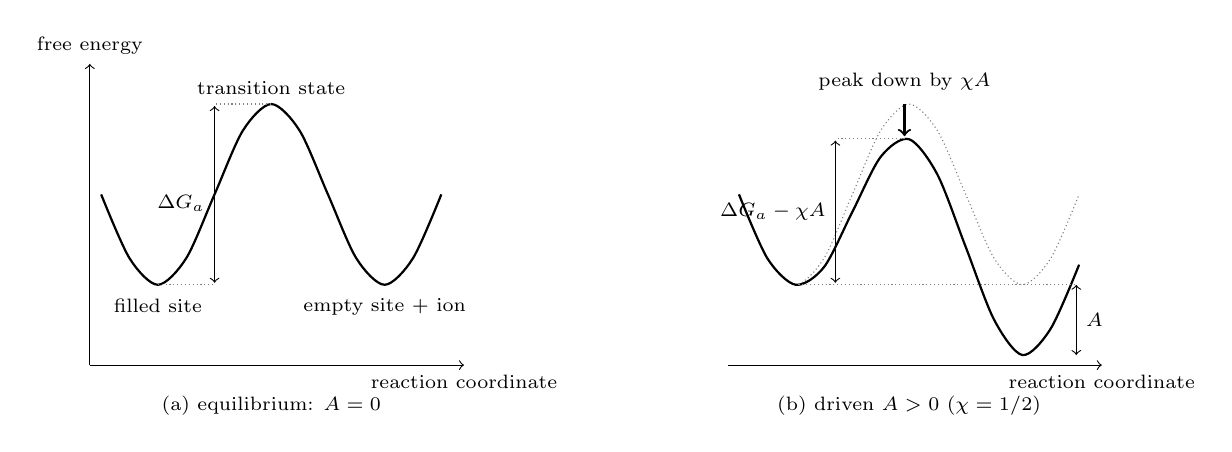
\begin{tikzpicture}[x=0.72cm,y=2.55cm]
% ---- (a) equilibrium landscape ----
\draw[->] (-0.2,-0.3) -- (6.4,-0.3) node[below,font=\scriptsize] {reaction coordinate};
\draw[->] (-0.2,-0.3) -- (-0.2,1.2) node[above,font=\scriptsize] {free energy};
\draw[thick] plot[smooth] coordinates {(0,0.55) (0.5,0.232) (1,0.1) (1.5,0.232) (2,0.55) (2.5,0.868) (3,1.0) (3.5,0.868) (4,0.55) (4.5,0.232) (5,0.1) (5.5,0.232) (6,0.55)};
\node[below,font=\scriptsize] at (1,0.08) {filled site};
\node[below,font=\scriptsize] at (5,0.08) {empty site + ion};
\node[above,font=\scriptsize] at (3,1.0) {transition state};
\draw[densely dotted,gray] (1,0.1) -- (2.0,0.1);
\draw[densely dotted,gray] (3,1.0) -- (2.0,1.0);
\draw[<->] (2.0,0.11) -- (2.0,0.99) node[pos=0.45,left,font=\scriptsize] {$\Delta G_a$};
\node[font=\scriptsize] at (3,-0.5) {(a) equilibrium: $A=0$};
\begin{scope}[xshift=8.1cm]
% ---- (b) driven landscape: A>0, chi=1/2 ----
\draw[->] (-0.2,-0.3) -- (6.4,-0.3) node[below,font=\scriptsize] {reaction coordinate};
\draw[densely dotted,thin,gray] plot[smooth] coordinates {(0,0.55) (0.5,0.232) (1,0.1) (1.5,0.232) (2,0.55) (2.5,0.868) (3,1.0) (3.5,0.868) (4,0.55) (4.5,0.232) (5,0.1) (5.5,0.232) (6,0.55)};
\draw[thick] plot[smooth] coordinates {(0,0.550) (0.5,0.232) (1,0.100) (1.5,0.188) (2,0.463) (2.5,0.737) (3,0.825) (3.5,0.649) (4,0.288) (4.5,-0.074) (5,-0.250) (5.5,-0.118) (6,0.200)};
\draw[->,thick] (2.92,1.0) -- (2.92,0.84) ;
\node[above,font=\scriptsize] at (2.92,1.02) {peak down by $\chi A$};
\draw[densely dotted,gray] (1.05,0.1) -- (1.7,0.1);
\draw[densely dotted,gray] (2.92,0.828) -- (1.7,0.828);
\draw[<->] (1.7,0.11) -- (1.7,0.818) node[pos=0.5,left,font=\scriptsize] {$\Delta G_a-\chi A$};
\draw[densely dotted,gray] (1.05,0.1) -- (5.95,0.1);
\draw[<->] (5.95,0.1) -- (5.95,-0.25) node[pos=0.5,right,font=\scriptsize] {$A$};
\node[font=\scriptsize] at (3,-0.5) {(b) driven $A>0$ ($\chi=1/2$)};
\end{scope}
\end{tikzpicture}
\caption{활성화 장벽 그림. (a) 평형 — 두 골짜기 같은 높이, 속도는 Eyring 식. (b) 구동력 $\mathcal A_j$ 가
도착 골짜기를 내리면 정방향 장벽 $\Delta G_a-\chi\mathcal A$, 역방향 $\Delta G_a+(1-\chi)\mathcal A$ 로 비대칭 이동
(식~\eqref{eq:bv}; 두 속도의 비가 식~\eqref{eq:db} detailed balance). 점선은 (a). 온도는 분모 $RT$ 로 진입.
이 그림이 식~\eqref{eq:xieq} logistic 과 \S\ref{sec:lag} 의 $L_q$ 두 결과의 공통 출발점이다.}
\label{fig:barrier}
\end{figure}

% ---- T5 (fig:flux) 원본 — 원 위치: ch1.tex L1291-1317 ----
\begin{figure}[t]
\centering
\begin{tikzpicture}[x=4.2cm,y=1.0cm]
\draw[-{Latex[length=1.4mm]}] (0,0) -- (0,2.35) node[above,font=\scriptsize] {flux [arb.]};
\draw[-{Latex[length=1.4mm]}] (-0.01,0) -- (1.1,0) node[below,font=\scriptsize] {$\xi$};
\foreach \xx in {0.5,1} {\draw (\xx,0.03) -- (\xx,-0.03) node[below,font=\scriptsize] {\xx};}
% forward r+ (1-xi): decreasing line from 2 to 0
\draw[thick] (0,2) -- (1,0);
% reverse r- xi: increasing line from 0 to 1
\draw[thick,densely dashed] (0,0) -- (1,1);
% A=0 pair (gray)
\draw[gray] (0,1.5) -- (1,0);
\draw[gray,densely dashed] (0,0) -- (1,1.5);
% intersection black: 2(1-xi)=xi -> xi=2/3
\draw[densely dotted] (0.6667,0) -- (0.6667,0.6667);
\fill (0.6667,0.6667) circle (0.9pt);
\node[below,font=\scriptsize] at (0.6667,-0.16) {$\xi_\eq$};
\fill[gray] (0.5,0.75) circle (0.9pt);
\node[right,font=\scriptsize] at (0.05,1.95) {forward $r^+(1-\xi)$};
\node[right,font=\scriptsize] at (0.75,0.55) {reverse $r^-\xi$};
\node[gray,font=\scriptsize] at (0.86,1.72) {gray: $A=0$};
\end{tikzpicture}
\caption{정지점 유도. 정방향 플럭스 $r^+(1-\xi)$(감소 직선)와 역방향 $r^-\xi$(증가 직선)의 교점이 정지점
$\xi_\eq$(식~\eqref{eq:logisticsolve}). $\mathcal A>0$($r^+=2r^-$, 검정)이면 $\xi_\eq=2/3$, $\mathcal A=0$
(회색)이면 $\tfrac12$ — detailed balance(식~\eqref{eq:db})가 평형을 정한다.}
\label{fig:flux}
\end{figure}

% ---- T6 (fig:logistic) 원본 — 원 위치: ch1.tex L1363-1385 ----
\begin{figure}[t]
\centering
\begin{tikzpicture}[x=1.05cm,y=1.0cm]
% left axis: xi_eq (S-curve), right: dxi/dV bell — shared z-axis
\draw[-{Latex[length=1.6mm]}] (-4.3,0) -- (4.5,0) node[below,font=\scriptsize] {$z=\sigma_d(V-U_j^{\,d})/w_j$};
\draw[-{Latex[length=1.6mm]}] (-4.3,0) -- (-4.3,3.4) node[above,font=\scriptsize] {$\xi_\eq$ \&\ $w\,|d\xi/dV|$};
\foreach \xx in {-4,-2,2,4} {\draw (\xx,0.04) -- (\xx,-0.04) node[below,font=\scriptsize] {\xx};}
\draw (-4.26,3.0) -- (-4.34,3.0) node[left,font=\scriptsize] {1};
\draw (-4.26,1.5) -- (-4.34,1.5) node[left,font=\scriptsize] {0.5};
% xi_eq = 1/(1+e^-z) scaled by 3
\draw[thick] plot[smooth] coordinates {(-4,0.0540) (-3,0.1423) (-2,0.3576) (-1,0.8068) (0,1.5) (1,2.1932) (2,2.6424) (3,2.8577) (4,2.9460)};
\node[right,font=\scriptsize] at (2.6,2.35) {$\xi_\eq$ (logistic)};
% derivative xi(1-xi) max 0.25 scaled by 3 -> max 0.75
\draw[densely dashed,thick] plot[smooth] coordinates {(-4,0.0530) (-3.5,0.0854) (-3,0.1355) (-2.5,0.2103) (-2,0.3150) (-1.5,0.4474) (-1,0.5898) (-0.5,0.7050) (0,0.7500) (0.5,0.7050) (1,0.5898) (1.5,0.4474) (2,0.3150) (2.5,0.2103) (3,0.1355) (3.5,0.0854) (4,0.0530)};
\node[right,font=\scriptsize] at (1.9,1.00) {$w\,|d\xi/dV|=\xi(1-\xi)$};
\draw[densely dotted] (0,0)--(0,0.75);
\node[below,font=\scriptsize] at (0,-0.32) {center $U_j^{\,d}$};
\end{tikzpicture}
\caption{평형 진행률과 그 미분. 실선 $=\xi_\eq$ logistic(식~\eqref{eq:xieq}), 파선 $=$ 폭으로 규격화한
미분 $w_j|d\xi_\eq/dV|=\xi_\eq(1-\xi_\eq)$ — $z=0$(중심 $U_j^{\,d}$)에서 최대 $\tfrac14$ 인 종 모양. 이 종이
다음 절의 평형 peak 이고, 방향에 불변(양수)이다.}
\label{fig:logistic}
\end{figure}

% ---- T7 (fig:reversal) 원본 — 원 위치: ch1.tex L1914-1946 ----
\begin{figure}[t]
\centering
\begin{tikzpicture}[x=1.05cm,y=0.95cm]
% discharge panel (left)
\begin{scope}
\draw[-{Latex[length=1.6mm]}] (-3.4,0) -- (3.4,0) node[below,font=\scriptsize] {$V$};
\draw[-{Latex[length=1.6mm]}] (-3.4,0) -- (-3.4,2.7) node[above,font=\scriptsize] {peak};
% bell (equilibrium) dotted
\draw[densely dotted,thick] plot[smooth] coordinates {(-3,0.27) (-2,0.66) (-1.5,1.04) (-1,1.55) (-0.5,2.02) (0,2.2) (0.5,2.02) (1,1.55) (1.5,1.04) (2,0.66) (3,0.27)};
% discharge tail: shifted/broadened to higher V (right)
\draw[thick] plot[smooth] coordinates {(-3,0.18) (-2,0.45) (-1.5,0.74) (-1,1.18) (-0.5,1.68) (0,2.0) (0.5,2.04) (1,1.78) (1.5,1.4) (2,1.02) (2.5,0.72) (3,0.5)};
\draw[-{Latex[length=1.4mm]},gray] (1.6,1.6)--(2.6,1.0);
\node[font=\scriptsize] at (1.7,2.0) {tail $\to$ higher $V$};
\node[font=\scriptsize,below] at (0,-0.42) {(a) discharge $\sigma_d=+1$: progress $V\uparrow$};
\end{scope}
% charge panel (right)
\begin{scope}[xshift=7.3cm]
\draw[-{Latex[length=1.6mm]}] (-3.4,0) -- (3.4,0) node[below,font=\scriptsize] {$V$};
\draw[-{Latex[length=1.6mm]}] (-3.4,0) -- (-3.4,2.7) node[above,font=\scriptsize] {peak};
\draw[densely dotted,thick] plot[smooth] coordinates {(-3,0.27) (-2,0.66) (-1.5,1.04) (-1,1.55) (-0.5,2.02) (0,2.2) (0.5,2.02) (1,1.55) (1.5,1.04) (2,0.66) (3,0.27)};
% charge tail: mirror — broadened to lower V (left)
\draw[thick] plot[smooth] coordinates {(-3,0.5) (-2.5,0.72) (-2,1.02) (-1.5,1.4) (-1,1.78) (-0.5,2.04) (0,2.0) (0.5,1.68) (1,1.18) (1.5,0.74) (2,0.45) (3,0.18)};
\draw[-{Latex[length=1.4mm]},gray] (-1.6,1.6)--(-2.6,1.0);
\node[font=\scriptsize] at (-1.5,2.0) {tail $\to$ lower $V$};
\node[font=\scriptsize,below] at (0,-0.42) {(b) charge $\sigma_d=-1$: progress $V\downarrow$ (grid reversed)};
\end{scope}
\end{tikzpicture}
\caption{인과 꼬리의 방향. 점선 $=$ 평형 종($\xi_\eq(1-\xi_\eq)/w$, 방향 불변). 실선 $=$ peak shape
with tail. (a) 방전은 진행이 $V\!\uparrow$ 라 꼬리가 높은 $V$ 쪽으로 늘어진다(격자 그대로). (b) 충전은 진행이
$V\!\downarrow$ 라 격자를 뒤집어 필터한 뒤 되돌려(역순 저역통과의 재역순) 꼬리가 낮은 $V$ 쪽으로 — 방전의 거울. 두 경우 모두
peak 는 양수.}
\label{fig:reversal}
\end{figure}

% ---- T8 (fig:widthbudget) 원본 — 원 위치: ch1.tex L1540-1568 ----
\begin{figure}[t]
\centering
\begin{tikzpicture}[x=0.72cm,y=22.0cm]
\draw[-{Latex[length=1.6mm]}] (-6.3,0) -- (10.8,0) node[below,font=\scriptsize] {$(V-U_j)/w_j$};
\draw[-{Latex[length=1.6mm]}] (-6.3,0) -- (-6.3,0.275) node[above,font=\scriptsize] {$\dd Q/\dd V$ (임의 단위)};
\foreach \xx in {-4,0,4,8} {\draw (\xx,0.004) -- (\xx,-0.004) node[below,font=\scriptsize] {\xx};}
% (0) equilibrium delta at plateau potential
\draw[-{Latex[length=1.8mm]},very thick] (0,0) -- (0,0.262);
\node[font=\scriptsize,align=center] at (-3.15,0.255) {평형 델타(Maxwell 전위)};
% (ii) intrinsic logistic-derivative bell, w=1
\draw[black!60] plot[smooth] coordinates {(-6,0.0025) (-5,0.0066) (-4,0.0177) (-3,0.0452) (-2,0.1050) (-1,0.1966) (-0.5,0.2350) (0,0.2500) (0.5,0.2350) (1,0.1966) (1.5,0.1491) (2,0.1050) (2.5,0.0701) (3,0.0452) (4,0.0177) (5,0.0066) (6,0.0025) (7,0.0009) (8,0.0003)};
\node[font=\scriptsize,black!60] at (2.55,0.205) {② 내재 $n_jRT/F$};
% (ii)x(iii) broadened bell, effective scale 1.6w
\draw[densely dashed] plot[smooth] coordinates {(-6,0.0140) (-5,0.0252) (-4,0.0438) (-3,0.0721) (-2,0.1082) (-1,0.1419) (-0.5,0.1525) (0,0.1562) (0.5,0.1525) (1,0.1419) (1.5,0.1264) (2,0.1082) (2.5,0.0895) (3,0.0721) (4,0.0438) (5,0.0252) (6,0.0140) (7,0.0077) (8,0.0042)};
\node[font=\scriptsize,align=left] at (-4.0,0.128) {②$\otimes$③ 분산 가법\\$\sigma_\eta=1.25\,\sigma_\mathrm{int}$, 유효 scale $1.6\,w_j$};
% (i) finite-rate skewed: C conv one-sided exp, L=1.5w
\draw[thick] plot[smooth] coordinates {(-6,0.0074) (-5,0.0134) (-4,0.0238) (-3,0.0408) (-2,0.0656) (-1,0.0959) (-0.5,0.1106) (0,0.1232) (0.5,0.1322) (1,0.1365) (1.5,0.1358) (2,0.1305) (2.5,0.1213) (3,0.1097) (4,0.0833) (5,0.0587) (6,0.0392) (7,0.0251) (8,0.0156) (9,0.0094) (10,0.0056)};
\draw[-{Latex[length=1.3mm]},gray] (4.4,0.093) -- (7.6,0.040);
\node[font=\scriptsize] at (6.8,0.098) {$+$① 지수 꼬리 $\ell=L_{V,j}$};
\end{tikzpicture}
\caption{두-상 broadening 의 폭 예산(식~\eqref{eq:widthbudget}; 좌표는 식 그대로의 수치 평가). 평형
델타(수직 화살)에 ② 내재 logistic 미분 종(폭 $w_j$, 가는 실선)이 얹히고, ③ 앙상블 $\eta$ 산포와의
합성곱이 분산 가법으로 종을 넓히며(예시 — $\eta$ 산포의 표준편차를 내재 몫의 $1.25$ 배로 두면
$\sigma_\mathrm{sym}=\sqrt{1+1.25^2}\,\sigma_\mathrm{int}\approx1.6\,\sigma_\mathrm{int}$, 같은
함수족이면 유효 scale $1.6w_j$ — 파선으로 표시), ① 유한율속이 한쪽 지수
꼬리(예시 $L_V=1.5w_j$ 와의 단측 합성곱 — 수치 적분)를 늘여 종을 소인 방향으로 민다(굵은 실선). 대칭
두 몫은 $w_j$ 하나에 흡수되고 비대칭 꼬리만 $L_{V,j}$ 로 분리된다.}
\label{fig:widthbudget}
\end{figure}
